% Generated from the same manifest as the project page.
\section{Current architectural evaluation}
\subsection{Protocol and architectural audit}
This cohort was captured with bevy\_zeroverse 0.32.0, generator 29, on 512 consecutive seeds (0--511), with 4 cameras per room, furnishing density 0.65 and static human density 0.25. Every audited room passed the recorded layout, support and camera-clearance checks. The first 32 rooms were rendered without appearance filtering at 640$\times$400, with 2 trajectory endpoints: 256 camera/time identities in six aligned modes. The audit contains 512 unique structural signatures after centimetre quantization; this bounded diagnostic does not estimate the total procedural space or learning utility.

\begin{table}[ht]\centering\small
\begin{tabular}{lrr}\toprule
Built feature & Rooms & Fraction \\\midrule
Arched portals & 194 / 512 & 37.9\% \\
Chamfered corners & 307 / 512 & 60.0\% \\
Exterior cut-in & 221 / 512 & 43.2\% \\
Interior pillars & 425 / 512 & 83.0\% \\
Mezzanine & 46 / 512 & 9.0\% \\
Oblique walls & 458 / 512 & 89.5\% \\
Raised floor & 90 / 512 & 17.6\% \\
Sloping ceiling & 354 / 512 & 69.1\% \\
Sunken floor & 103 / 512 & 20.1\% \\
\bottomrule\end{tabular}
\caption{Architectural features in the complete consecutive population. Features co-occur; fractions do not sum to 100\%.}\label{tab:architecture}
\end{table}

\subsection{Geometry, calibration and displayed captures}
Footprint areas span 35.05--262.58 m$^2$, with roof pitch 0.00--11.32$^\circ$. Figure~\ref{fig:architecture-levels} and Figure~\ref{fig:architecture-envelopes} pair native RGB with the actual serialized envelope plans and sections. Camera arrows indicate direction, rather than frusta. Solid furnishings are footprint proxies; the sections show roof and floor levels and omit furnishings, pillars and partitions. Structural feature examples are selected independently of rendered appearance; all rooms remain available in the contact sheet and explorer. Metric constraints are not building-code certification.

The page presents all 32 rooms, all four cameras and both endpoints in one explorer, with 1536 channel images. RGB, depth, normals, semantics, positions, co-visibility, camera calibration and plans share the same room/time identity. RGB preserves renderer tone mapping and sRGB encoding without per-image exposure correction or cropping. All previews use lossless WebP. Depth is an 8-bit axial-depth preview divided by 15 m and clamped; normals store $(n+1)/2$, and positions are affine-normalized by the annotation AABB and clamped. Semantic colors are preserved exactly. These previews are not float32 training labels. Geometric annotations use the first surface, including opaque glass, rather than reflected or refracted optical content.

The native capture protocol uses Auto quality, shadows, SSAO and approximate diffuse GI with 1024 primary rays per probe. Renderer identity and capabilities are recorded in every calibration download. All captured views passed the recorded alignment checks: maximum per-view depth/position p99 error 2.861 $\mu$m, reprojection p99 0.00076 pixels and normal-length error 2.384e-7. Every view contains at least 6 semantic classes. 16/16 rooms with humans in the camera's primary functional zone show person pixels; 3/21 rooms with humans anywhere in the main envelope never show person pixels. These are class-level observations, rather than instance-level visibility guarantees.

Scene construction through capture/export takes 1.94--4.11 seconds per room (median 3.06), excluding application startup. This is a bounded capture run, not a sustained-throughput, unlimited-process memory-stability or photographic-realism qualification.

\begin{figure}[p]
\centering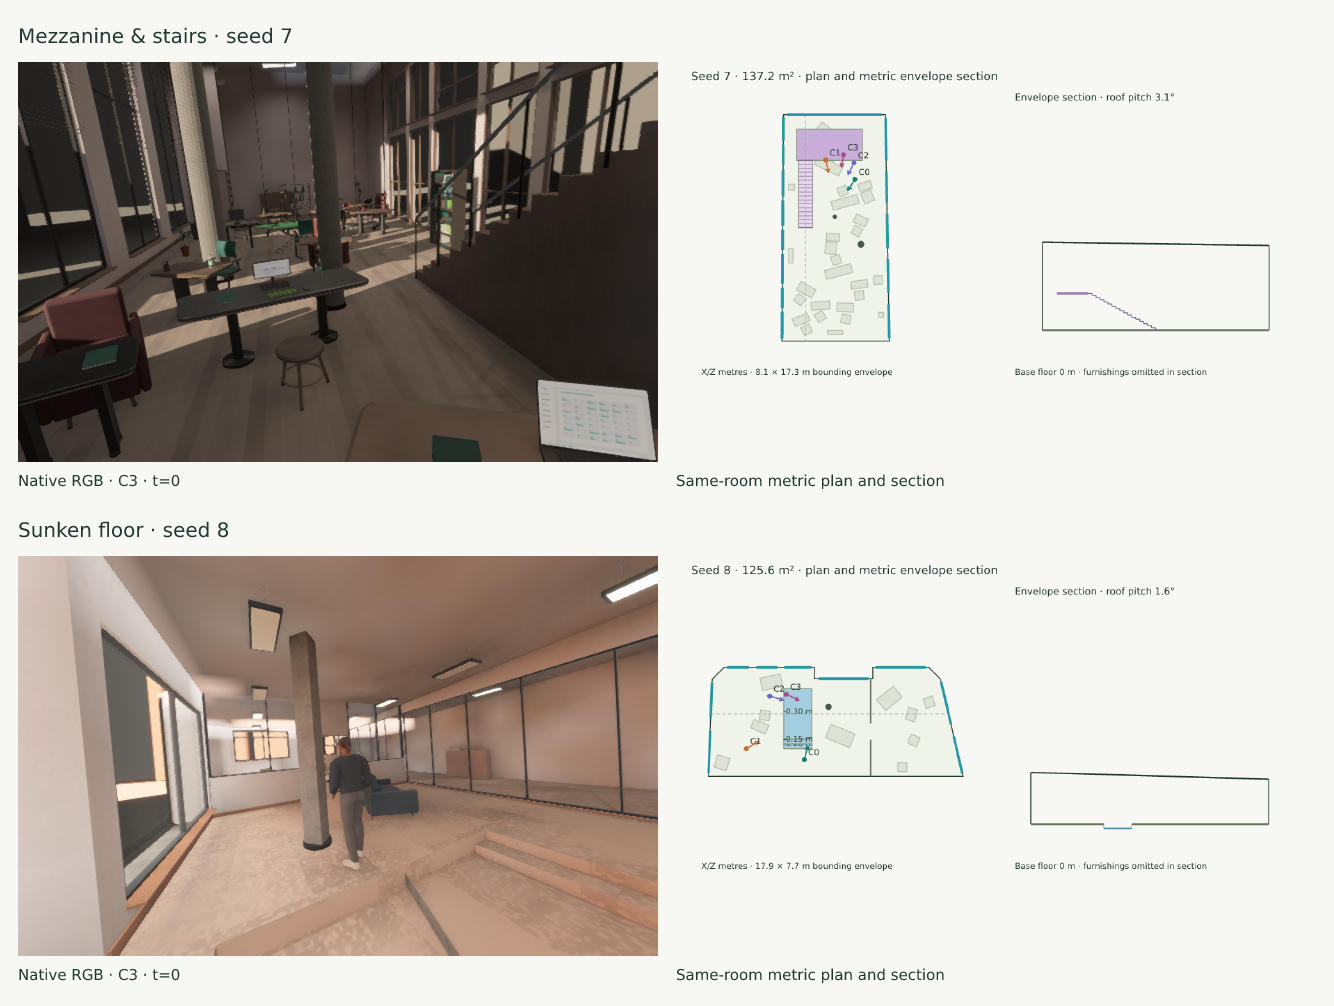
\includegraphics[width=\linewidth,height=.82\textheight,keepaspectratio]{generated/architecture_levels.jpg}
\caption{Native RGB and metric plans of structurally selected rooms. Raised and depressed levels, decks and stairs are generated geometry. Cyan marks glazing; orange/blue denote raised/sunken floors; violet denotes mezzanines and stairs.}\label{fig:architecture-levels}
\end{figure}

\begin{figure}[p]
\centering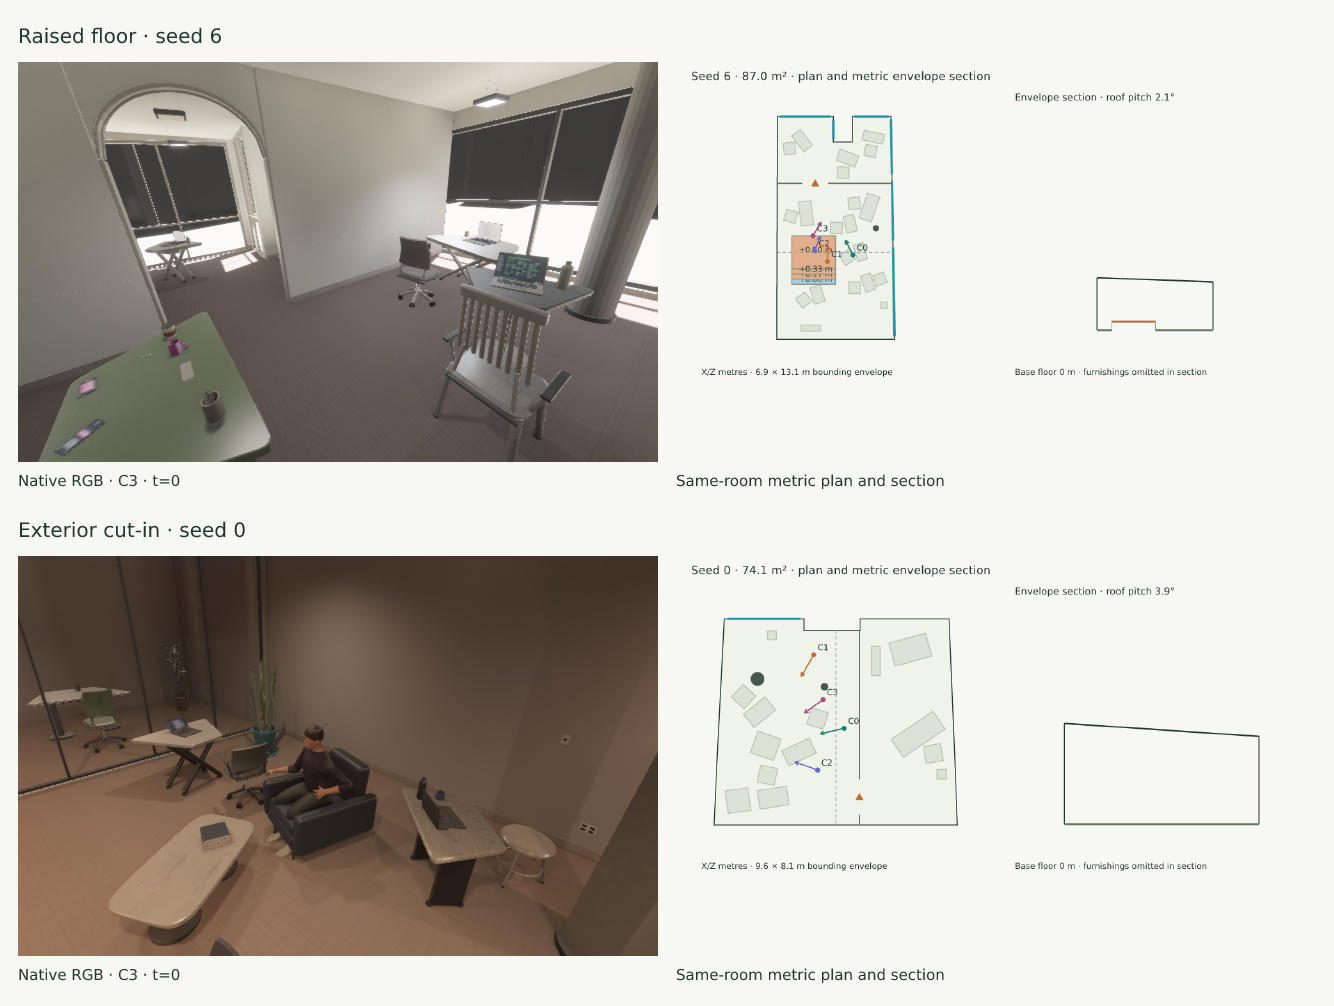
\includegraphics[width=\linewidth,height=.82\textheight,keepaspectratio]{generated/architecture_envelopes.jpg}
\caption{Native RGB paired with the corresponding envelope programs. Floor levels, portals, polygonal outlines and apertures vary; features can be outside a particular camera view.}\label{fig:architecture-envelopes}
\end{figure}

\begin{figure}[p]
\centering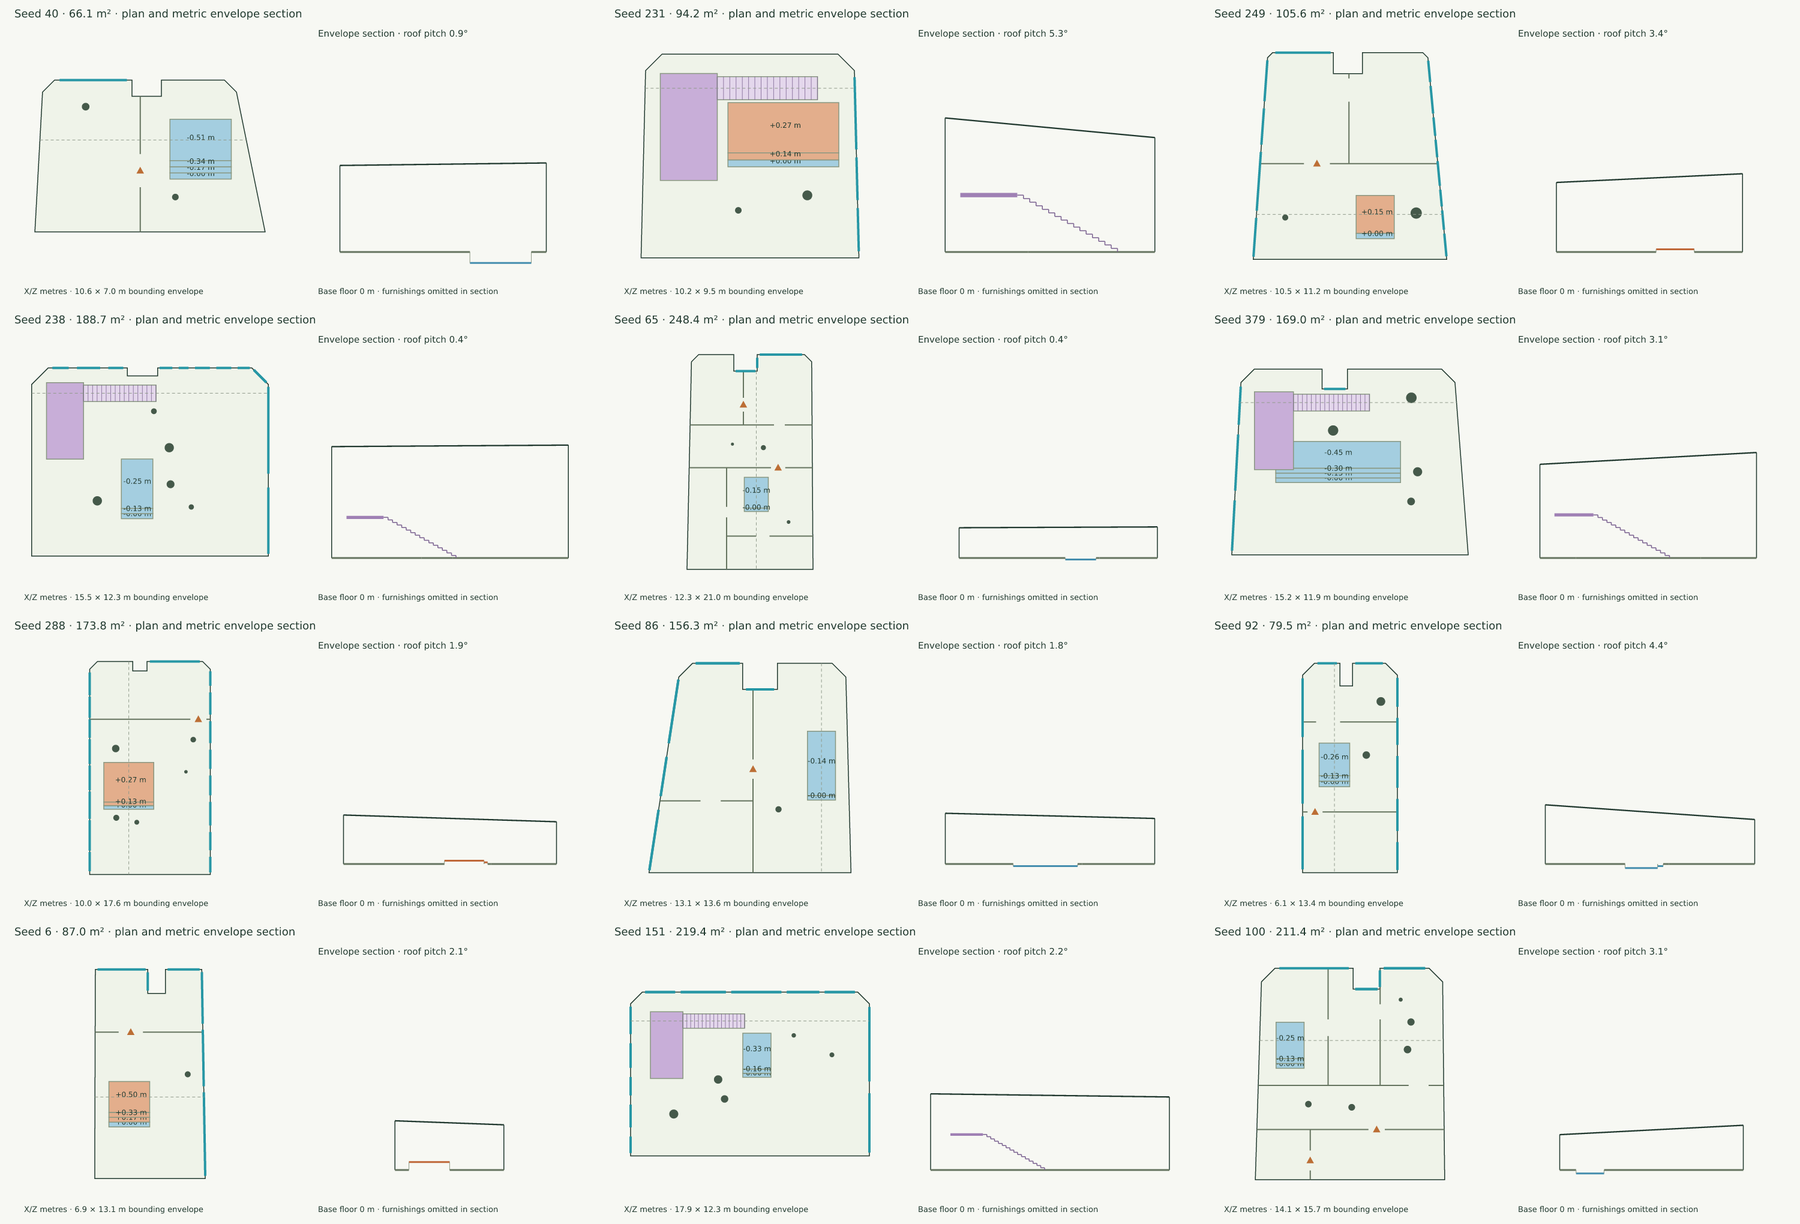
\includegraphics[width=\linewidth,height=.82\textheight,keepaspectratio]{generated/architecture_footprints.png}
\caption{Twelve metric envelope programs selected by architectural feature coverage from the full consecutive population. Plans are diagrams, not twelve additional RGB renders.}\label{fig:architecture-plans}
\end{figure}

\begin{figure}[p]
\centering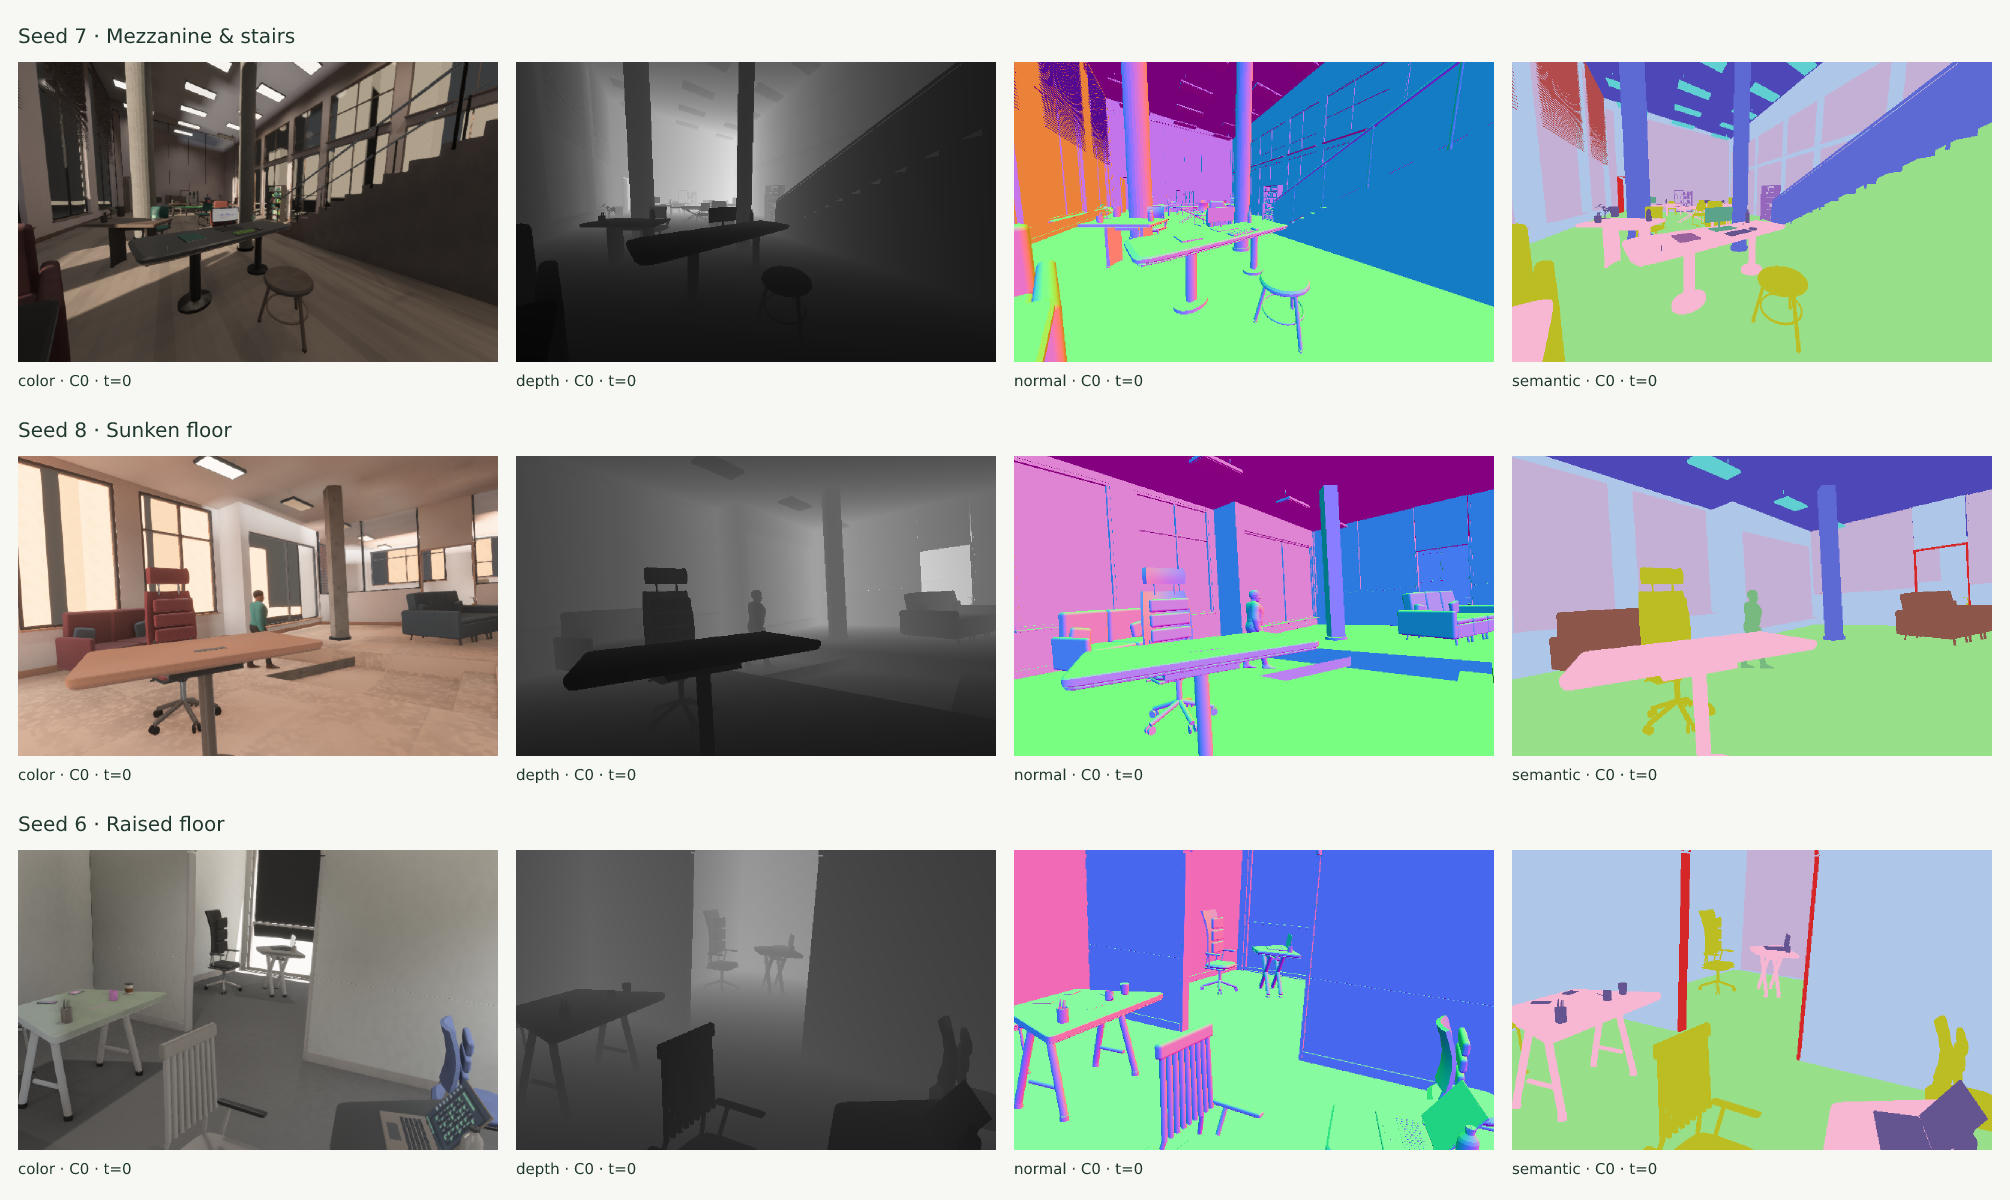
\includegraphics[width=\linewidth,height=.82\textheight,keepaspectratio]{generated/architecture_annotations.jpg}
\caption{Matched RGB, depth, view-space normals and semantic display previews, camera 0 at t=0. All six annotations, camera identities and endpoint times remain accessible in the explorer.}\label{fig:architecture-annotations}
\end{figure}

\subsection{Co-visibility in every captured room}
Production co-visibility accompanies every RGB and geometry view in this cohort. Each valid source pixel stores an exact uint16 membership mask of other capture cameras that see its first surface, with the source bit excluded. One deterministic additive legend is shared across all views. The unified explorer supports all memberships and individual-peer overlays; the selected peer's own tile stays RGB.

Across every room and endpoint, 82.7\% of valid source-pixel observations are visible to at least one peer. This pixel-weighted statistic pools 65535995 valid source-pixel observations; it does not count unique 3D points. Exact downloads include 16-bit grayscale membership PNGs, separate 8-bit 0/1 validity PNGs, calibrated transforms and the ordered camera legend. Zero membership with valid=1 is an unshared surface; zero membership with valid=0 is background. Co-visibility and other annotations were captured together, rather than joined from separate runs.

\begin{figure}[p]
\centering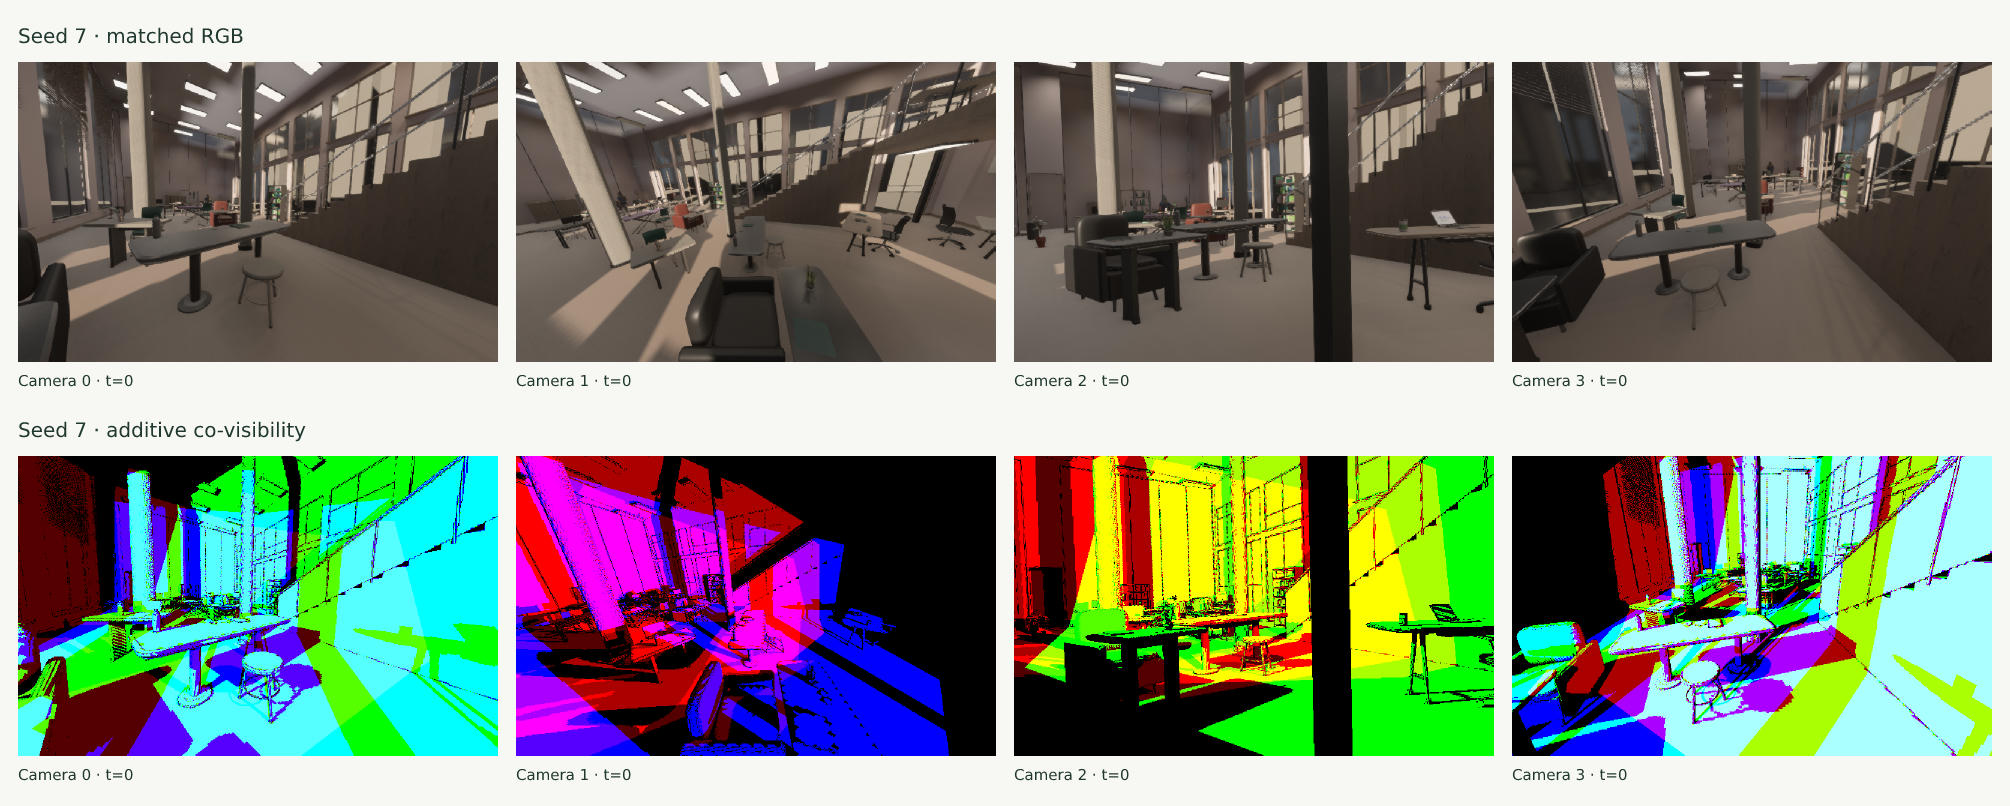
\includegraphics[width=\linewidth,height=.82\textheight,keepaspectratio]{generated/architecture_co_visibility.jpg}
\caption{Seed 7 at t=0: four native RGB views above their production co-visibility annotations. Columns retain the same camera/time identity. All captured rooms expose this annotation in the same explorer.}\label{fig:architecture-co-visibility}
\end{figure}

\subsection{Matched camera and appearance qualification}
A separate prespecified factor sweep covers 2 geometry families, eleven settings, two cameras and two timestamps per variant (88 RGB images). Room geometry hashes are invariant across each family's camera, material, detail, illumination and exposure interventions. People are disabled in this sweep. The receipt binds the actual native executable, source identity, target, feature flags and locked package versions. All cases are retained, including failures; no model inference filters pairs. The project page provides the complete matched annotation gallery and machine-readable receipt.

New captures export a full row-major pixel-space $K$, image dimensions, half-pixel centers, a versioned centered pinhole lens contract, normalized playback progress, eased trajectory progress and optional explicitly assigned seconds. Unassigned physical time remains unknown. Short handheld paths sample local metric translations and yaw/pitch/roll increments independently of a moving look-target, retaining swept collision checks. Requested high/low/zero proxy-overlap strata are selected before placement retries. Their all-ray proxy estimates are stored separately from rendered directed overlap over valid source pixels. A proxy-negative pair can retain a small rendered overlap. Lens distortion and sampled principal points are not implemented.

Table~\ref{tab:factor-qualification} reports means over directed rendered pairs, and the maximum per-view 99th-percentile self-reprojection error. There are 10 exact duplicate RGB images: the baseline/overlap interventions deliberately reuse the reference camera. These counts measure exact repetition in this matched study, not perceptual redundancy across a training population. Sensor white balance, blur, noise and optional JPEG are separate seeded RGB-only export transforms with individual operator regressions; they are not applied in this render sweep. This bounded check does not establish photographic realism, a calibrated sensor model, a fitted training mixture or downstream transfer.

\begin{table}[htbp]\centering\small
\begin{tabular}{lrrr}\toprule
Factor & Shared pixels (\%) & Baseline (m) & Reproj. p99 max (px) \\
\midrule
reference & 57.0981 & 1.704 & 0.00010 \\
portrait & 50.5508 & 2.019 & 0.00013 \\
wide baseline & 49.9170 & 4.385 & 0.00010 \\
handheld & 43.2062 & 2.743 & 0.00010 \\
low overlap & 10.7074 & 2.363 & 0.00007 \\
no proxy overlap & 0.0000 & 1.876 & 0.00010 \\
material seed & 57.0981 & 1.704 & 0.00010 \\
low detail & 57.0981 & 1.704 & 0.00010 \\
lighting seed & 57.0981 & 1.704 & 0.00010 \\
dim illumination & 57.0981 & 1.704 & 0.00010 \\
exposure & 57.0981 & 1.704 & 0.00010 \\
\bottomrule\end{tabular}
\caption{Prespecified factor checks on matched room geometry. Directed overlap uses valid source pixels; the zero target refers to placement proxies.}\label{tab:factor-qualification}
\end{table}

\subsection{Population distributions and publication contract}
Room and object counts retain zero-instance rooms. Camera and photometric histograms state their own sample denominators. Placement heatmaps use 33 path samples per camera and normalize each panel independently. Feature shortcuts do not change population denominators. A seed's bit width and continuous parameter ranges do not establish ten-million-sample diversity; correlations, placement constraints and rendering affect distinguishable outcomes. Frozen SigLIP2 embeddings support separate redundancy audits, but no embedding-rank or downstream-learning result is claimed here.

The project page, paper, figures and calibration archives are built by a single Rust publication pipeline from one completed capture manifest. A compiled generator identity binds crate version, geometry grammar and source/dependency hashes. The publisher validates scene/camera/time identities, every requested channel, exact membership masks, annotation checks and population denominators before staging artifacts. The release/deployment gate checks input and output hashes, preserving explicitly separate historical reference studies. Author-written method text and measurements have distinct roles; publication attestation does not imply photographic or downstream validation.

\begin{figure}[p]
\centering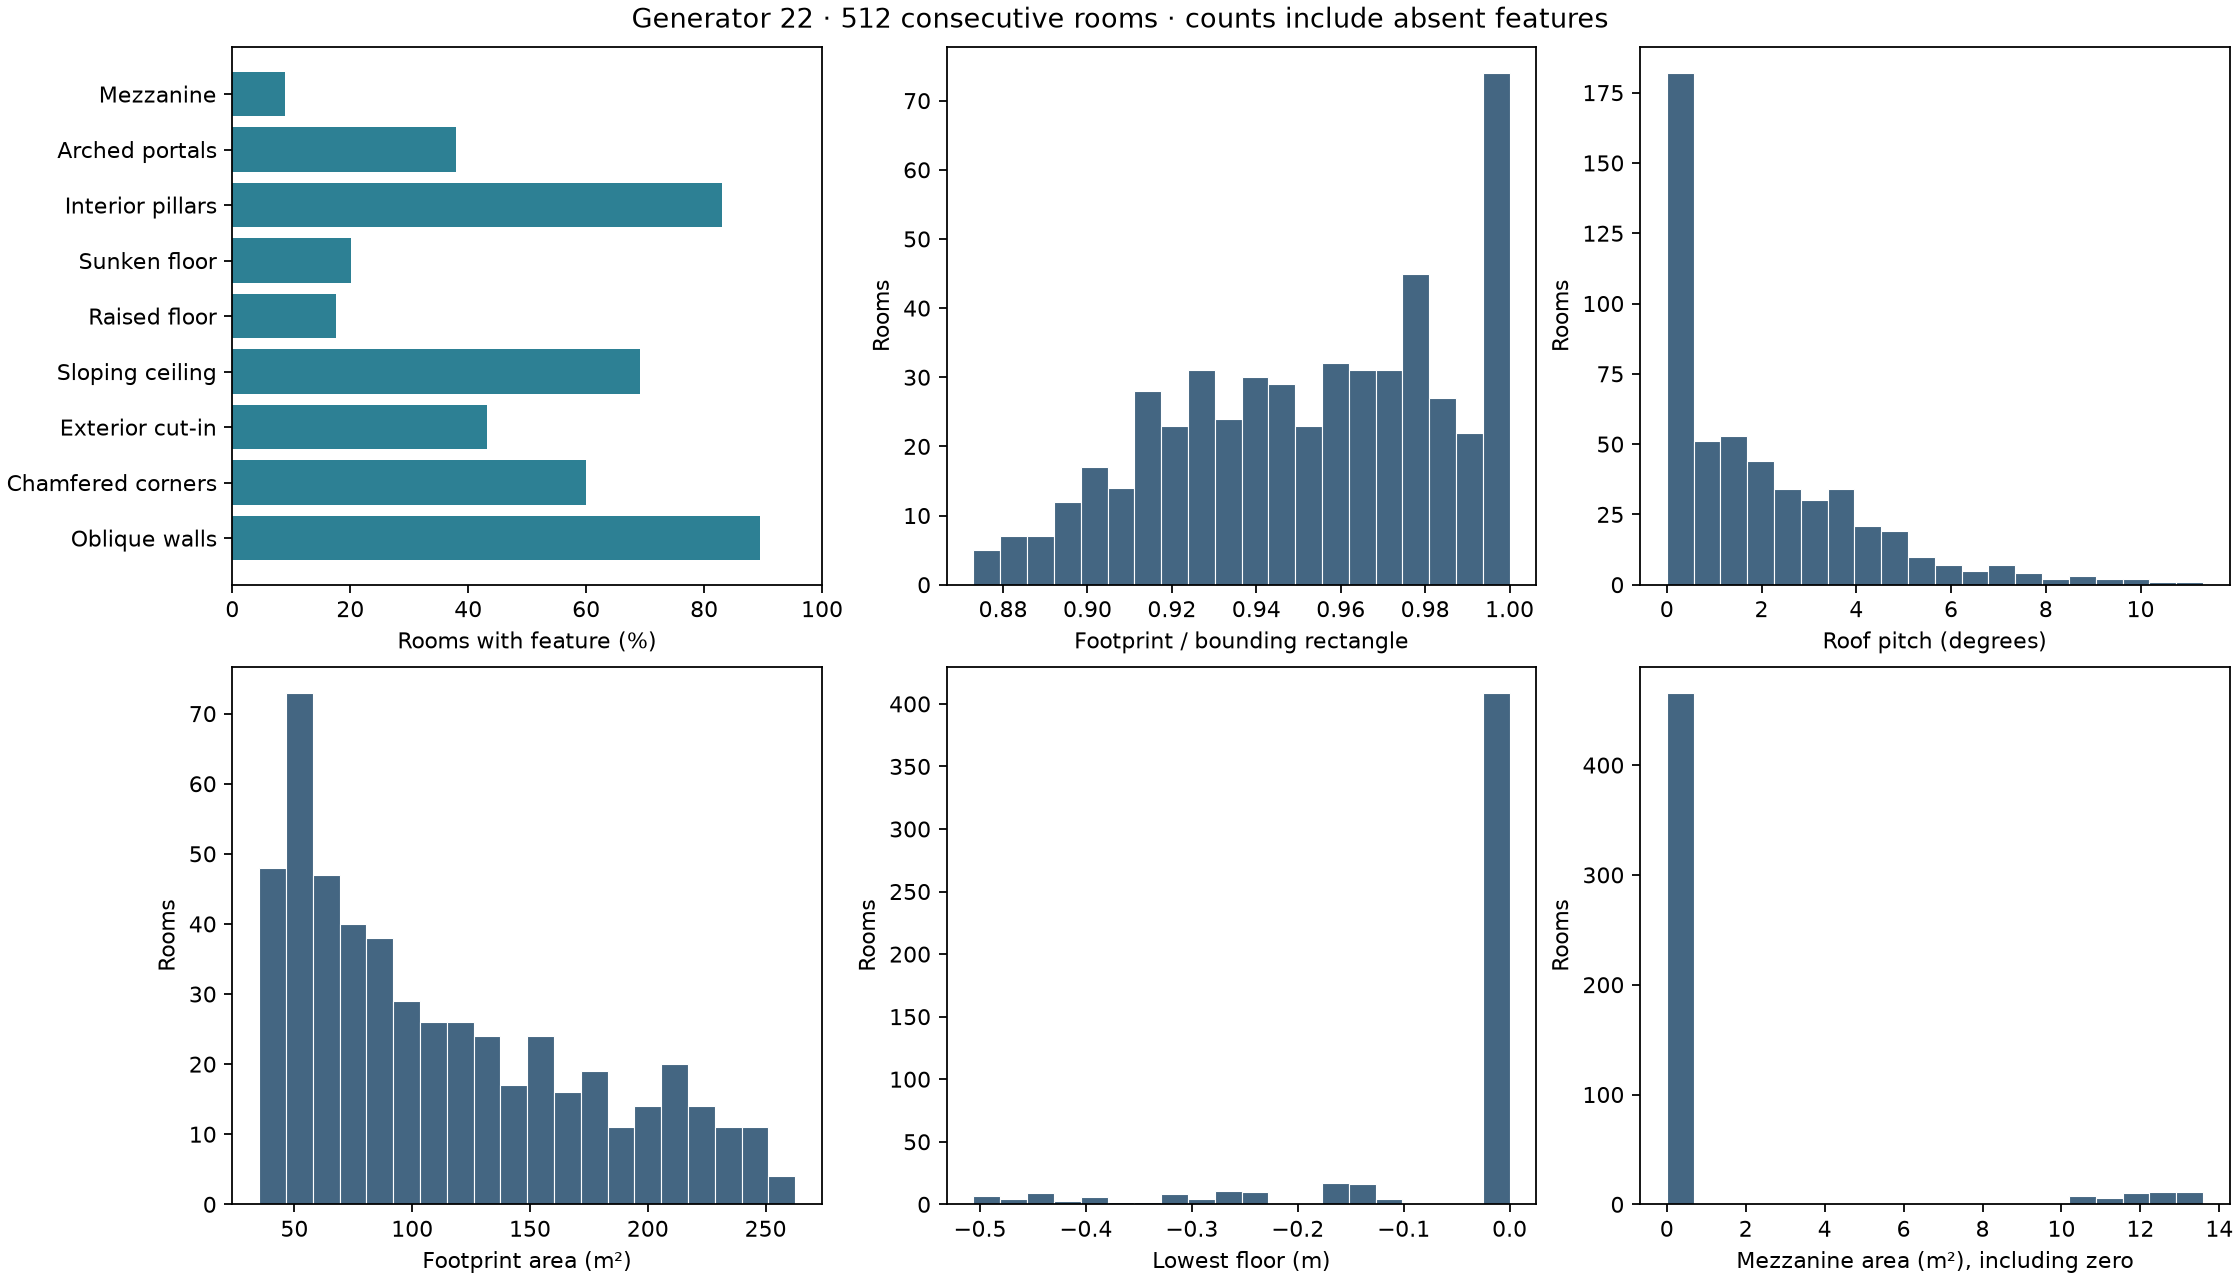
\includegraphics[width=\linewidth,height=.82\textheight,keepaspectratio]{generated/architecture_features.png}
\caption{Architectural feature counts and continuous parameter distributions from the complete population; absent features are retained.}\label{fig:architecture-features}
\end{figure}

\begin{figure}[p]
\centering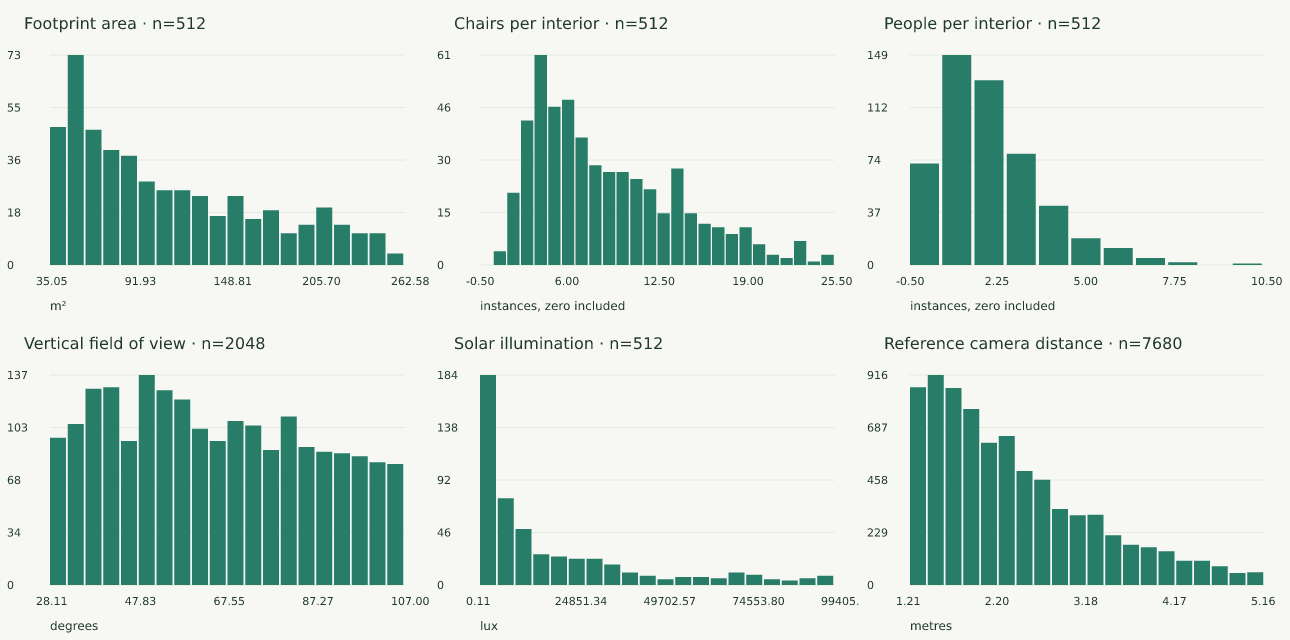
\includegraphics[width=\linewidth,height=.82\textheight,keepaspectratio]{generated/architecture_population.png}
\caption{Furnishing, lighting and camera variation in the same population. Every panel states its denominator.}\label{fig:architecture-population}
\end{figure}

\begin{figure}[p]
\centering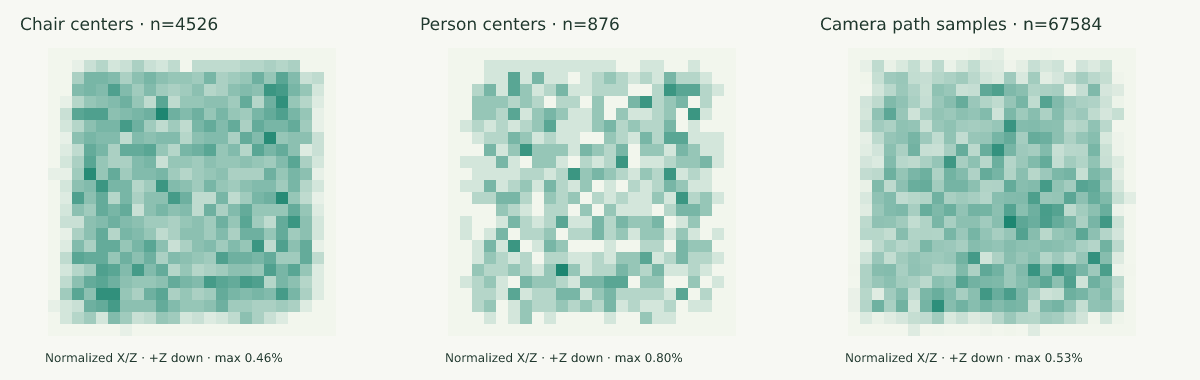
\includegraphics[width=\linewidth,height=.82\textheight,keepaspectratio]{generated/architecture_placement.png}
\caption{Chair centers, human centers and camera path samples in normalized room X/Z coordinates, with +Z down. Each panel reports its own sample count and color scale.}\label{fig:architecture-placement}
\end{figure}

\begin{figure}[p]
\centering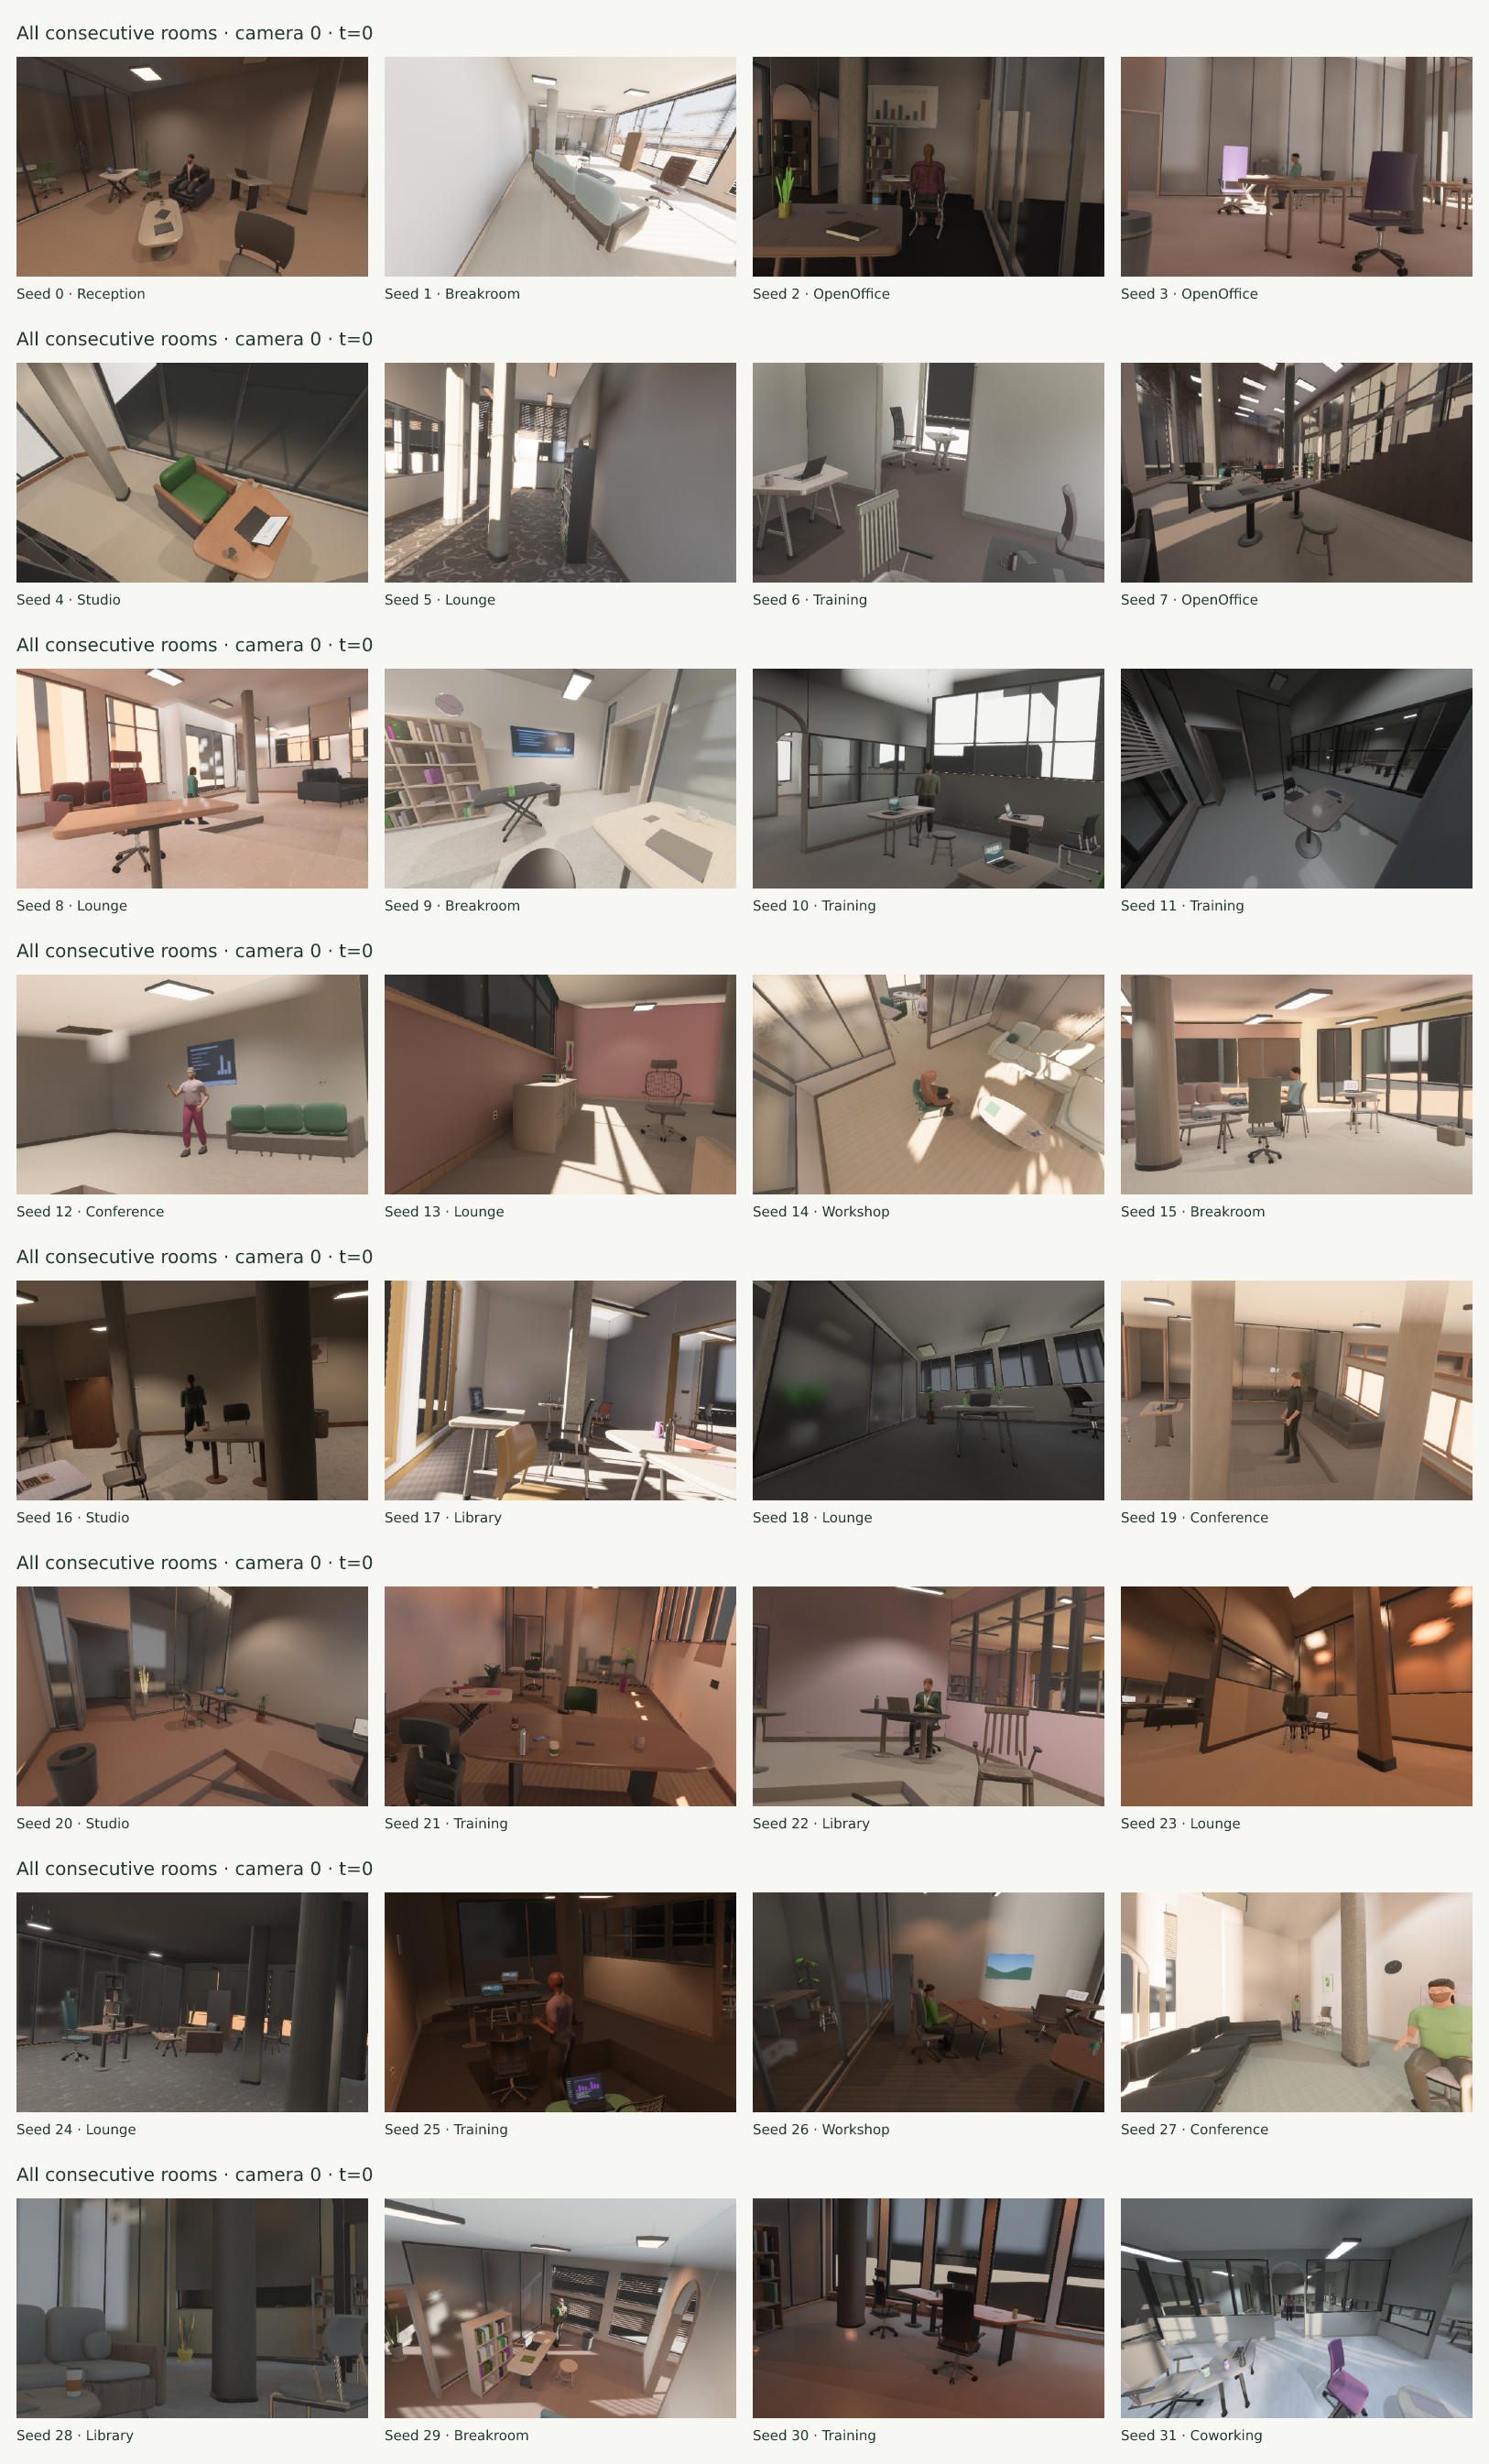
\includegraphics[width=\linewidth,height=.82\textheight,keepaspectratio]{generated/architecture_consecutive.jpg}
\caption{Every consecutively rendered room, camera 0 at t=0, including dark and sparsely furnished rooms. All four cameras, endpoints and six modes remain in the project-page explorer.}\label{fig:architecture-consecutive}
\end{figure}

\clearpage
